\documentclass[a0paper,portrait]{baposter}


%\usepackage[latin1]{inputenc}   % UNIX, codage ISO 8859-1
\usepackage[english,french]{babel}   % "babel.sty" + "french.sty"
\usepackage[utf8]{inputenc}
\usepackage{relsize}		% For \smaller
\usepackage{url}			% For \url
\usepackage{epstopdf}	% Included EPS files automatically converted to PDF to include with pdflatex
\usepackage{amsmath}
\usepackage{amsmath,graphicx,cite,amssymb}
\usepackage{array}
\usepackage{xkeyval}
%%% Global Settings %%%%%%%%%%%%%%%%%%%%%%%%%%%%%%%%%%%%%%%%%%%%%%%%%%%%%%%%%%%

\graphicspath{{Figures/}}	% Root directory of the pictures 
\tracingstats=2			% Enabled LaTeX logging with conditionals

%%% Color Definitions %%%%%%%%%%%%%%%%%%%%%%%%%%%%%%%%%%%%%%%%%%%%%%%%%%%%%%%%%

\definecolor{bordercol}{RGB}{0,0,0}
\definecolor{headercol1}{RGB}{0,0,0}
\definecolor{headercol2}{RGB}{0,0,0}
\definecolor{headerfontcol}{RGB}{255,255,255}
\definecolor{bgcol}{RGB}{197,3,71}
\definecolor{boxcolor}{RGB}{255,255,255}

\newcommand{\argmin}{\operatornamewithlimits{argmin}}
\newcommand{\argmax}{\operatornamewithlimits{argmax}}
\newcommand*\E{\ensuremath{\textup{e}}\xspace}
		
%%%%%%%%%%%%%%%%%%%%%%%%%%%%%%%%%%%%%%%%%%%%%%%%%%%%%%%%%%%%%%%%%%%%%%%%%%%%%%%%
%%% Utility functions %%%%%%%%%%%%%%%%%%%%%%%%%%%%%%%%%%%%%%%%%%%%%%%%%%%%%%%%%%

%%% Save space in lists. Use this after the opening of the list %%%%%%%%%%%%%%%%
\newcommand{\compresslist}{
	\setlength{\itemsep}{1pt}
	\setlength{\parskip}{0pt}
	\setlength{\parsep}{0pt}
}

%%%%%%%%%%%%%%%%%%%%%%%%%%%%%%%%%%%%%%%%%%%%%%%%%%%%%%%%%%%%%%%%%%%%%%%%%%%%%%%
%%% Document Start %%%%%%%%%%%%%%%%%%%%%%%%%%%%%%%%%%%%%%%%%%%%%%%%%%%%%%%%%%%%
%%%%%%%%%%%%%%%%%%%%%%%%%%%%%%%%%%%%%%%%%%%%%%%%%%%%%%%%%%%%%%%%%%%%%%%%%%%%%%%

\begin{document}
\typeout{Poster rendering started}

%%% Setting Background Image %%%%%%%%%%%%%%%%%%%%%%%%%%%%%%%%%%%%%%%%%%%%%%%%%%
\background{
	\begin{tikzpicture}[remember picture,overlay]%
	\draw (current page.north west)+(-2em,2em) node[anchor=north west]
	{
\includegraphics[height=1.1\textheight]{background-red}};
	\end{tikzpicture}
}

%%% General Poster Settings %%%%%%%%%%%%%%%%%%%%%%%%%%%%%%%%%%%%%%%%%%%%%%%%%%%
%%%%%% Eye Catcher, Title, Authors and University Images %%%%%%%%%%%%%%%%%%%%%%
\begin{poster}{
	grid=false,
	% Option is left on true though the eyecatcher is not used. The reason is
	% that we have a bit nicer looking title and author formatting in the headercol
	% this way
	eyecatcher=true, 
	borderColor=bordercol,
	headerColorOne=headercol1,
	headerColorTwo=headercol2,
	headerFontColor=headerfontcol,
	% Only simple background color used, no shading, so boxColorTwo isn't necessary
	boxColorOne=boxcolor,
	headershape=roundedright,
	headerfont=\Large\textsf,
	headerheight=0.1\textheight,
	textborder=roundedleft,
	background=user,
	bgColorOne=bgcol,
	bgColorTwo=bgcol,
	headerborder=closed,
  boxshade=plain,
  boxpadding=1em,
  boxheaderheight=2em,
  cornerradius= 1em,
  colspacing= 1em,
  columns=2,
  grid=false,
}
%%% Eye Cacther %%%%%%%%%%%%%%%%%%%%%%%%%%%%%%%%%%%%%%%%%%%%%%%%%%%%%%%%%%%%%%%
{
	\setlength\fboxsep{0pt}
	\setlength\fboxrule{0.5pt}
	\fbox{
			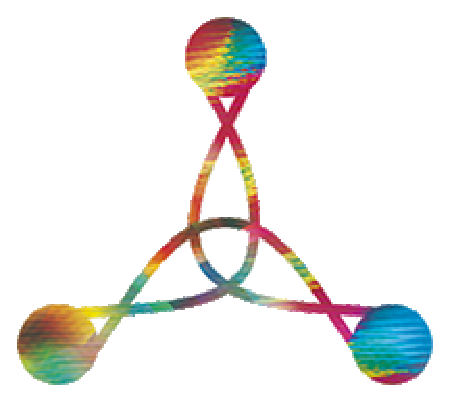
\includegraphics[scale=0.2]{logo-gretsi}
	}
		
}	
%%% Title %%%%%%%%%%%%%%%%%%%%%%%%%%%%%%%%%%%%%%%%%%%%%%%%%%%%%%%%%%%%%%%%%%%%%
{ \bf \\ 
	\huge \textcolor{white}{Méthode structurée de décomposition en matrices non-négatives appliquée à la séparation de sources audio}
}
%%% Authors %%%%%%%%%%%%%%%%%%%%%%%%%%%%%%%%%%%%%%%%%%%%%%%%%%%%%%%%%%%%%%%%%%%
{ \sf \large
	\vspace{0em} \textcolor{white}{Cl\'{e}ment LAROCHE, Matthieu KOWALSKI,\\ H\'{e}l\`{e}ne PAPADOPOULOS, Ga\"{e}l RICHARD}\\
	{\sf \normalsize \textcolor{white}{Institut Mines-T\'el\'ecom - T\'el\'ecom ParisTech - CNRS/LTCI , France}}\\
    {\sf \normalsize \textcolor{white}{Univ Paris-Sud-CNRS-CentraleSupelec, L2S, France}}\\
%	{\sf \vspace{0.3cm} \textcolor{white}{paul.magron@telecom-paristech.fr}}
\vspace{0em}

}
%%% Logo %%%%%%%%%%%%%%%%%%%%%%%%%%%%%%%%%%%%%%%%%%%%%%%%%%%%%%%%%%%%%%%%%%%%%%
{
% The logos are compressed a bit into a simple box to make them smaller on the result
% (Wasn't able to find any bigger of them.)
\setlength\fboxsep{0pt}
\setlength\fboxrule{0.5pt}
%	\fbox{
			
\includegraphics[scale=0.15]{logo_tpt}
			
\includegraphics[scale=0.15]{logo-universite-Paris_Sud}
%	}
}


\headerbox{\textbf{Introduction}}{name=intro,column=0,row=0}{

\large\textbf{Objectif} \normalsize \\ 
Séparer les instruments harmoniques des instruments percussifs d'un signal audio monophonique. \\


\textcolor{bgcol}{$\bullet$} Les instruments harmoniques possèdent des spectres parcimonieux (spectres à bande étroite).\\
\textcolor{bgcol}{$\bullet$} Les instruments percussifs sont des signaux transitoires à large bande. \\

\large\textbf{Approche proposée} \normalsize \\
Idée principale : tirer profit de la parcimonie de la décomposition NMF projetée (PNMF) : \\
\textcolor{bgcol}{$\rightarrow$} \textit{Parcimonie Spectrale} de la partie harmonique intrinsèque à la PNMF. \\
\textcolor{bgcol}{$\rightarrow$} Partie NMF classique pour traduire les composantes mal représentées par la partie orthogonale (i.e., spectres à large bande). \\
\textcolor{bgcol}{$\rightarrow$} Peu de paramètres à optimiser. \\
\vspace{-1em} 
}



\headerbox{\textbf{Lien entre la PNMF et les méthodes actuelles}}{name=horiz,column=0,below=intro}{

\large\textbf{Lien entre la NMF et la PNMF} \normalsize \\ 
\vspace*{-1em}

Problème NMF : 
\begin{equation}
\min_{W,H\geqslant0} \| V - WH \|^{2} ,
\end{equation}
Problème PNMF : 
\vspace{-1mm}
\begin{equation}
\min_{W\geqslant0} \| V - WW^{T}V \|^{2}
\end{equation}
avec $V$ la matrice de données $\in \mathbb{R}_+^{n \times m}$, $W$ la matrice dictionnaire $\in \mathbb{R}_+^{n \times k}$, $H$ la matrice d'activation $\in \mathbb{R}_+^{k \times m}$ \\

\textcolor{bgcol}{$\bullet$} Dans la PNMF, la matrice $H$ est remplacée par $W^TV$. \\







\large\textbf{Lien entre la PNMF et la PCA} \normalsize \\ 
\vspace*{-1em}

\textcolor{bgcol}{$\bullet$} En retirant la contrainte de non-négativité à la PNMF, on obtient un problème de PCA classique où la solution est une matrice orthogonale composée des vecteurs propres de $VV^T$. \\

}




\headerbox{\textbf{NMF projetée structurée (SPNMF)}}{name=onset,column=0,below=horiz,above=bottom}{


\large\textbf{Séparation Harmonique/Percussif} \normalsize \\
%\vspace*{-1em}

Le problème s'écrit de la façon suivante : 
\begin{equation}
V \approx W_{1}H_{1} + W_{2} H_{2},
\end{equation}  
avec : \\
\textcolor{bgcol}{$\bullet$} $W_{1}H_{1}$ est la partie presque orthogonale de rang $k'$, \\
\textcolor{bgcol}{$\bullet$} $ W_{2} H_{2} $ sont $e$ composantes NMF qui constituent la partie percussive. \\


\large\textbf{Contrainte de la PNMF} \normalsize \\ 
%\vspace*{-1em}

On pose ensuite la contrainte de la PNMF : $H_{1} =  W_{1}^{T} (V - W_{2} H_{2})$ ssi $W_{1}^{T}W_1 = I$ .
Ce qui nous donne la fonction de coût : 
\begin{equation}\label{cout}
\min_{W_1,W_2,H_2\geq 0} || V - W_{1}W_{1}^{T} (V - W_{2} H_{2}) - W_{2} H_{2} ||^{2}.
\end{equation}
\vspace{-1em}



\large\textbf{Optimisation} \normalsize \\ 
%\vspace*{-1em}

Règles de mise à jour multiplicative :\\
Soit $F$ la fonction de coût associée à \eqref{cout}. \\
\textcolor{bgcol}{$\bullet$} $\nabla F(W_1) = [\nabla F(W_{1})]^{+} - [\nabla F(W_{1})]^{-}$  \\
\vspace*{+0.3em}

\textcolor{bgcol}{$\bullet$} $W_{1} \leftarrow W_{1} \otimes \frac{ [\nabla F(W_{1})]^{-} }{[\nabla F(W_{1})]^{+}}. $ \\

\textcolor{bgcol}{$\bullet$} Optimisation alternée entre $W_1$, $W_2$ et $H_2$. \\

\vspace*{-0.5em}

}

\headerbox{\textbf{Benchmark de notre méthode}}{name=experiment,span=1,column=1,row=0}{

\large\textbf{Résultats expérimentaux synthétiques} \normalsize \\ 
\vspace*{0em}
Spectrogramme de notre signal synthétique de test : % composé d'un Do ($131$Hz), d'un Sol ($196$Hz) et de $0.1$s de bruit blanc toute les $1$s pour simuler un instrument percussif. 
\begin{center}
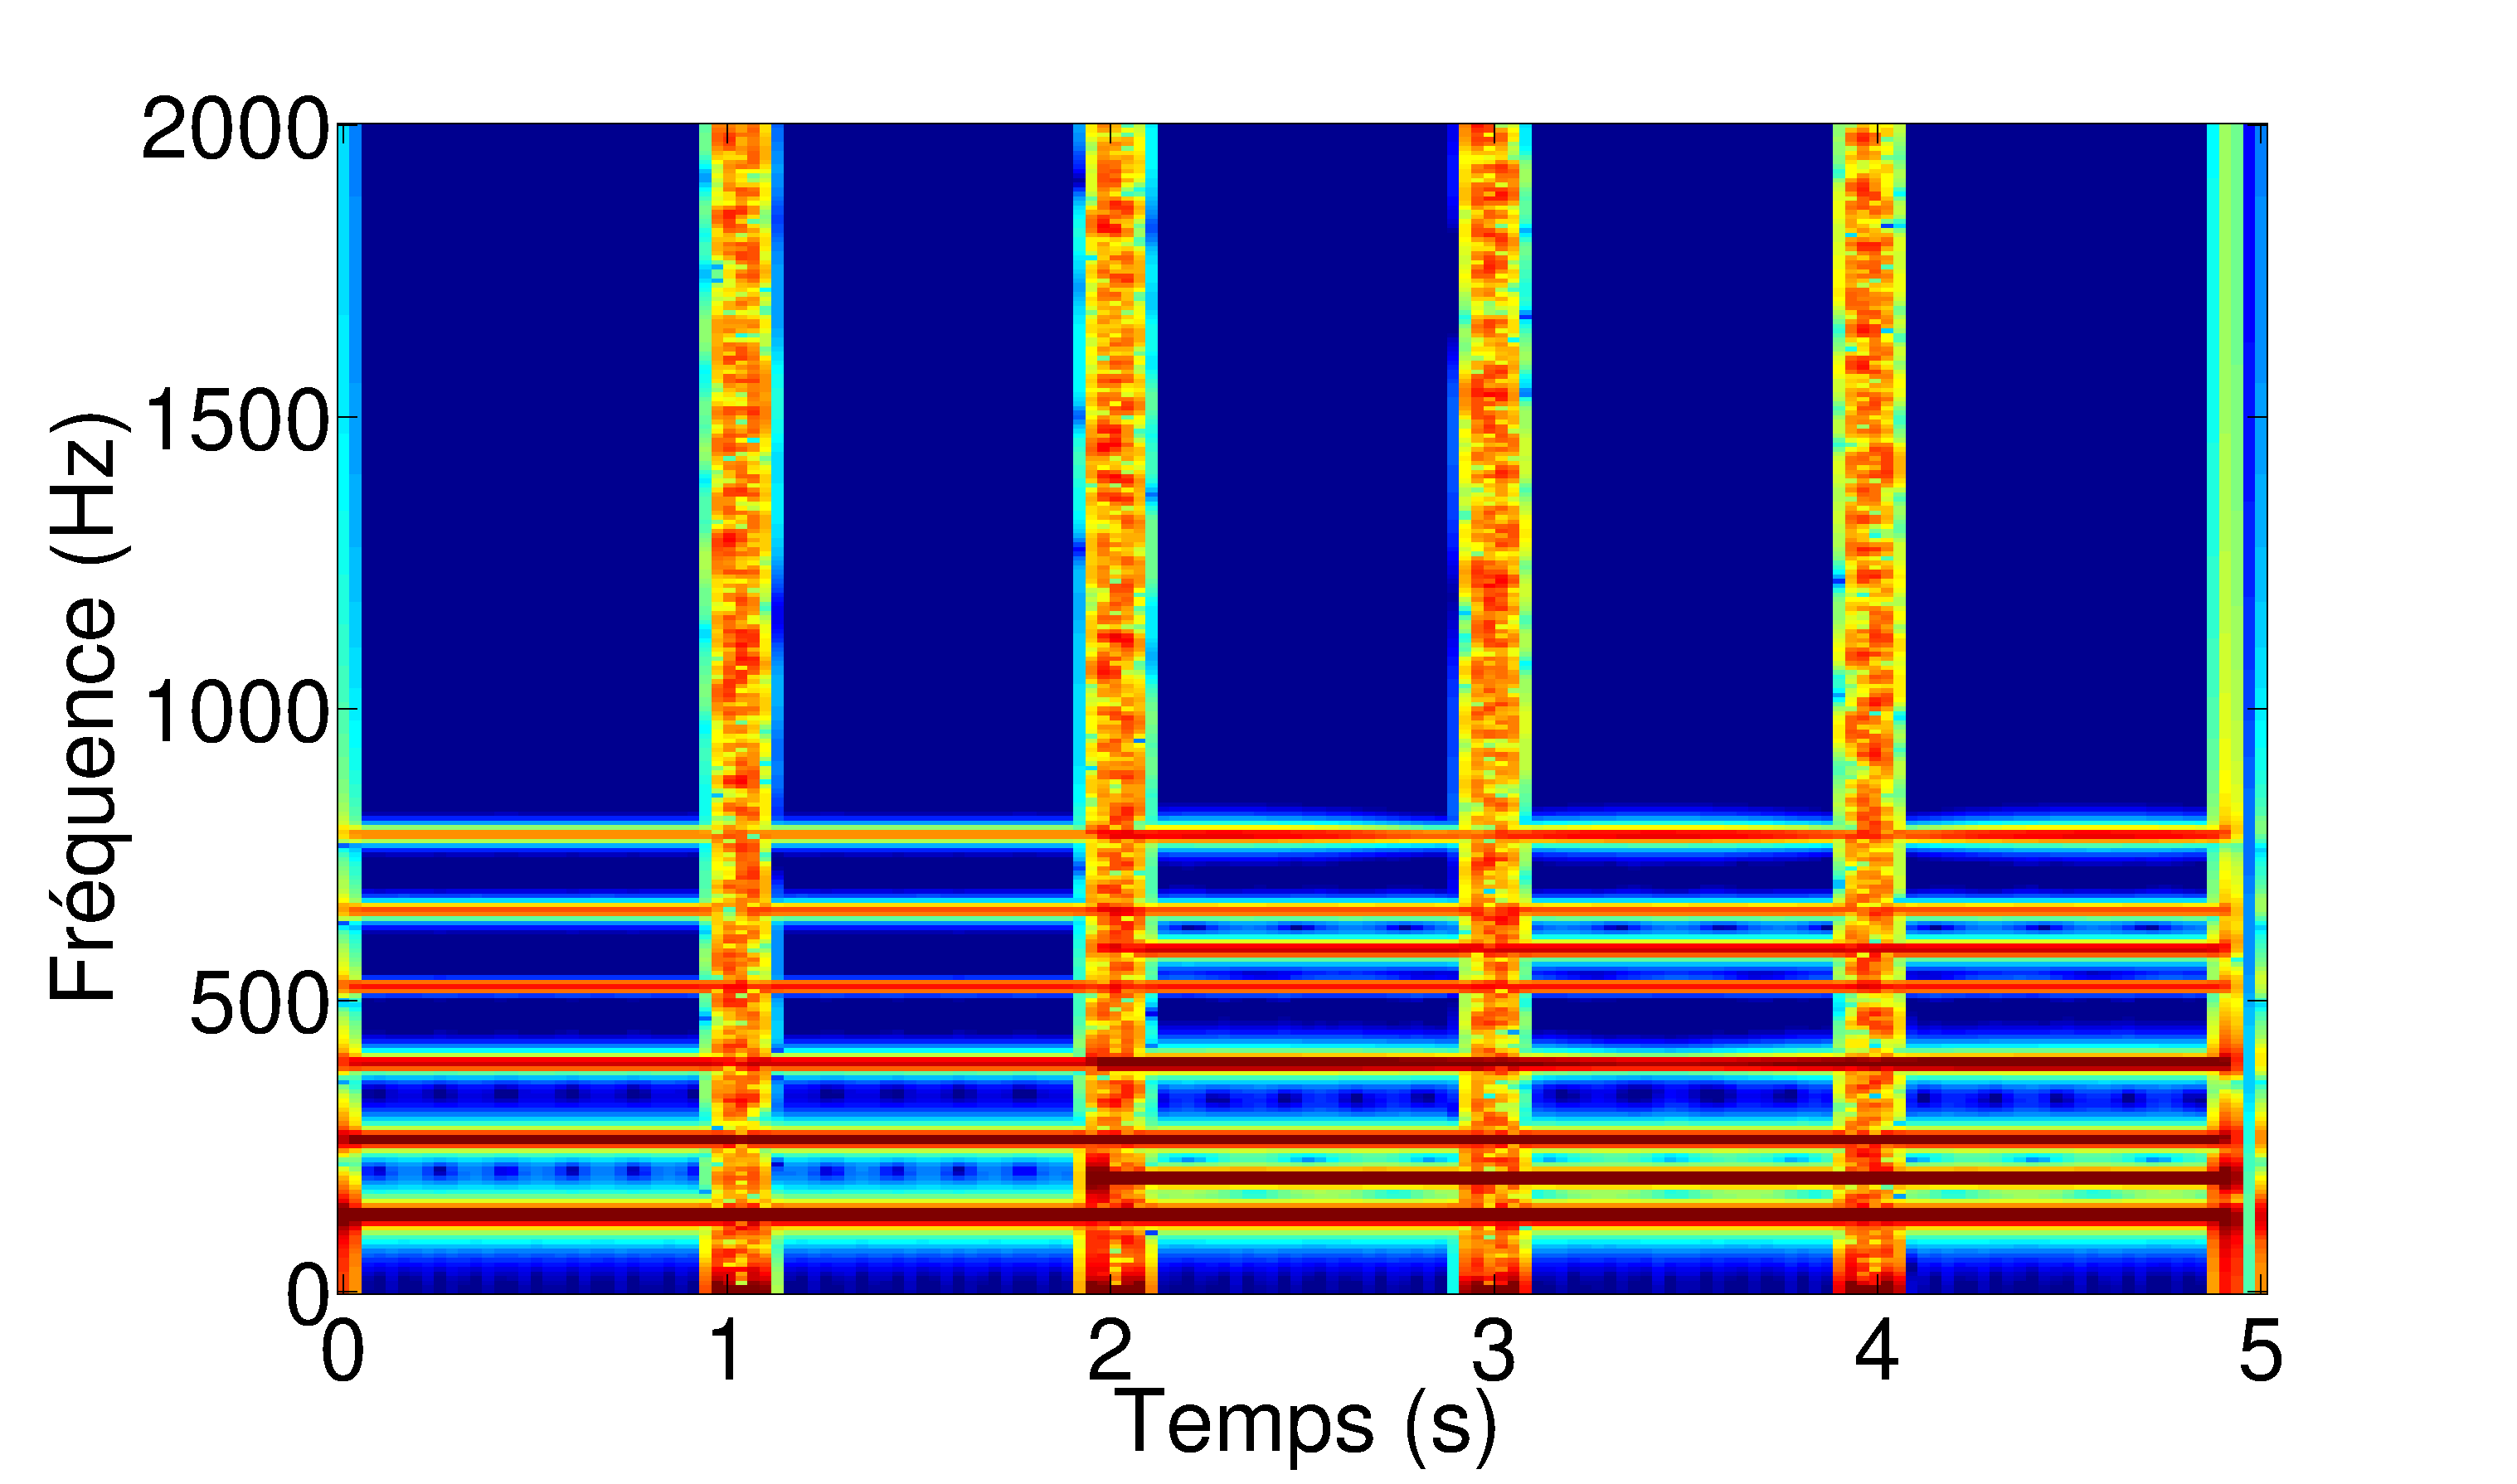
\includegraphics[scale=0.13]{testsynth}
\end{center}
\vspace{-0.5em}

\textcolor{bgcol}{$\bullet$} Simulation d'une séparation harmonique/percussive sur un signal synthétique. \\
\textcolor{bgcol}{$\bullet$} Validation de notre algorithme lors d'un recouvrement dans le domaine temps-fréquence. \\
\textcolor{bgcol}{$\bullet$} Qualité de reconstruction du signal mesurée avec les métriques usuelles~: Rapport Signal-Distorsion (RSD), Rapport Signal-Artefact (RSA), Rapport Signal-Interférence (RSI). \\
\vspace{-0.5em}
\begin{center}
   \begin{tabular}{|c|c|c|c|}
  \hline
  RSD  & NMF(dB) & PNMF(dB) & SPNMF(dB) \\
  \hline
  C(3)  & 11.21 & 7.97   & \textbf{13.44} \\
  G(3)  & 10.44   & \textbf{13.16}  & 11.55 \\
  Noise   & 2.37  & 0.11 & \textbf{12.54} \\  
  \hline
  RSI & NMF(dB) & PNMF(dB) & SPNMF(dB) \\
  \hline
 C(3) & \textbf{30.85}   & 17.67    &  21.66  \\
 G(3) & 13.45   & 4.94   &  \textbf{29.30}  \\
 Noise & 4.62  &  0.45  &  \textbf{14.36} \\
 \hline
  RSA & NMF(dB) & PNMF(dB) & SPNMF(dB) \\
  \hline
 C(3) & 9.4   & \textbf{23.3} &   20.0 \\
 G(3) & 10.3  & 15.2 &  \textbf{18.3}  \\
 Noise & 16.0 & 10.2 &  \textbf{16.3} \\
 \hline  
\end{tabular} 
\end{center}

}

\headerbox{\textbf{Comparaison à l'état de l'art}}{name=resto,span=1,column=1,below=experiment}{
        
Comparaison à l'état de l'art en utilisant le protocole expérimental détaillé dans \cite{NMFC}. \\

\vspace{-1em}
\begin{center}
\begin{tabular}{|c | c c c | c c c |}
  \hline
  &\multicolumn{3}{|c|}{NMF contrainte \cite{NMFC}} & \multicolumn{3}{|c|}{SPNMF} \\
  \hline
Séparation percussive & RSD & RSI  & RSA & RSD & RSI & RSA \\ \hline
T2\textunderscore 01 & 4.0 & 6.5 & \textbf{5.7} & \textbf{4.3} & \textbf{11.0} & 5.6  \\
T2\textunderscore 02 & \textbf{5.2} & 8.3 & \textbf{7.5} & 5.0 & \textbf{9.7} & 7.2  \\
T2\textunderscore 03 & \textbf{2.8} & 2.6 & \textbf{11.1} & 1.5 & \textbf{6.6} & 4.0 \\
T2\textunderscore 04 & \textbf{7.5} & \textbf{10.3} & \textbf{10.3} & 3.6 & 6.5 & 7.7 \\ \hline
Moyenne & \textbf{4.9} & 7.0 & \textbf{8.7} & 3.6 & \textbf{8.4} & 6.1 \\
 \hline

 Séparation harmonique & RSD & RSI  & RSA & RSD & RSI & RSA \\ \hline
T2\textunderscore 01 & \textbf{11.0} & \textbf{14.8} & 13.9 & 7.3 & 7.4  & \textbf{28.3} \\
T2\textunderscore 02 & \textbf{7.5} & \textbf{9.3} & 12.1 & 6.5 & 7.8 & \textbf{12.8} \\
T2\textunderscore 03 & \textbf{5.0} & \textbf{9.1} & \textbf{8.6} & 3.8 & 6.2 & 8.4 \\
T2\textunderscore 04 & \textbf{7.5} & \textbf{10.6} & \textbf{10.5} & 4.7 & 6.6 & 10.1 \\ \hline
Moyenne & \textbf{7.8} & \textbf{11.0} & 11.3 & 5.6 & 7.0 & \textbf{14.9} \\
 \hline
\end{tabular}
\end{center}

\textcolor{bgcol}{$\bullet$} La NMF contrainte obtient de meilleurs résultats, cependant la méthode nécessite une optimisation couteuse (6 paramètres) et dépendante des signaux traités. \\
\vspace{-1.5em} 
}



\headerbox{\textbf{Travaux futurs}}{name=conclusion,span=1,column=1,below=resto,above=bottom}{

\textcolor{bgcol}{$\bullet$} Stratégie d'initialisation de la partie percussive (NMF informée). \\
\textcolor{bgcol}{$\bullet$} Utilisation d'une matrice dictionnaire pour la partie percussive. \\
\textcolor{bgcol}{$\bullet$} Comparaison de la SPNMF à la méthode de \cite{NMFC} sur une base de données plus grande. \\

\vspace{-0.5em} 

Références:
% Bibliographie
\footnotesize 											% Make the whole text smaller
\bibliographystyle{IEEEbib}							% Use plain style
\renewcommand{\section}[2]{\vskip 0.05em}		% Omit "References" title
\begin{thebibliography}{1}							% Simple bibliography with widest label of 1
\itemsep=-0.01em										% Save space between the separation
\setlength{\baselineskip}{0.4em}					% Save space with longer lines


\bibitem{NMFC} F. Canadas-Quesada and P. Vera-Candeas and N. Ruiz-Reyes and J. Carabias-Orti and P. Cabanas-Molero, Percussive/harmonic sound separation by non-negative matrix factorization with smoothness/sparseness constraints, EURASIP Journal on Audio, Speech, and Music Processing, 2014.
%\bibitem{bsseval} E. Vincent and R. Gribonval and C. F\'{e}votte, Performance measurement in blind audio source separation, IEEE Trans. Audio, Speech, Language Process., 2006.
\end{thebibliography}

}

\end{poster}
\end{document}